\chapter{ANALISIS}
\section{System Definition}
\begin{figure}[h]
	\centering
	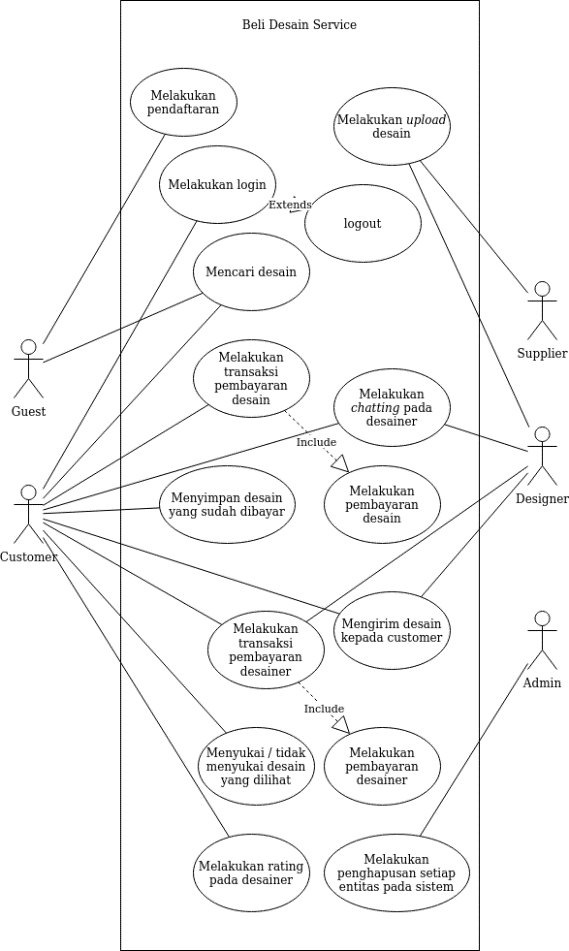
\includegraphics{usecase}
	\caption{Use Case Diagram Sistem Belidesain}
\end{figure}

\section{Identifikasi Permasalahan}
Berdasarkan latar belakang yang telah ditulis, terdapat beberapa identifikasi masalah yang dapat disimpulkan yaitu sebagai berikut:
\begin{enumerate}
	\item Penjualan desain pada platform \textit{e-commerce} jarang ditemui.
	\item Penyebaran informasi pameran desain yang belum meluas.
	\item Pencarian jasa desainer panggilan masih jarang ditemui.
\end{enumerate}

\section{Identifikasi Kebutuhan Pengguna}
Berdasarakan latar belakang yang telah ditulis, berikut terdapat beberapa identifikasi kebutuhan pengguna:
\begin{enumerate}
	\item Dapat menemukan desain yang cocok dengan selera
	\item Dapat membeli desain dengan mudah dan cepat
	\item Dapat menyimpan desain yang dibeli untuk memudahkan pengaksesan
	\item Dapat berkomunikasi atau berkonsultasi dengan desainer
	\item Dapat meminta desainer untuk membuatkan desain yang diinginkan
	\item Dapat melakukan upload dan mempublikasi desain yang dibuat
\end{enumerate}
